\chapter*{Appendix A: Code Access} \label{code_data}
\addcontentsline{toc}{chapter}{Appendix A}
All relevant code and data can be found on the GitHub repository: https://github.com/BirkTorpmannHagen/Master

\chapter*{Appendix B: p-values}\label{p-values}
\addcontentsline{toc}{chapter}{Appendix B: p-values}

\begin{figure}[hbt]
    \centering
    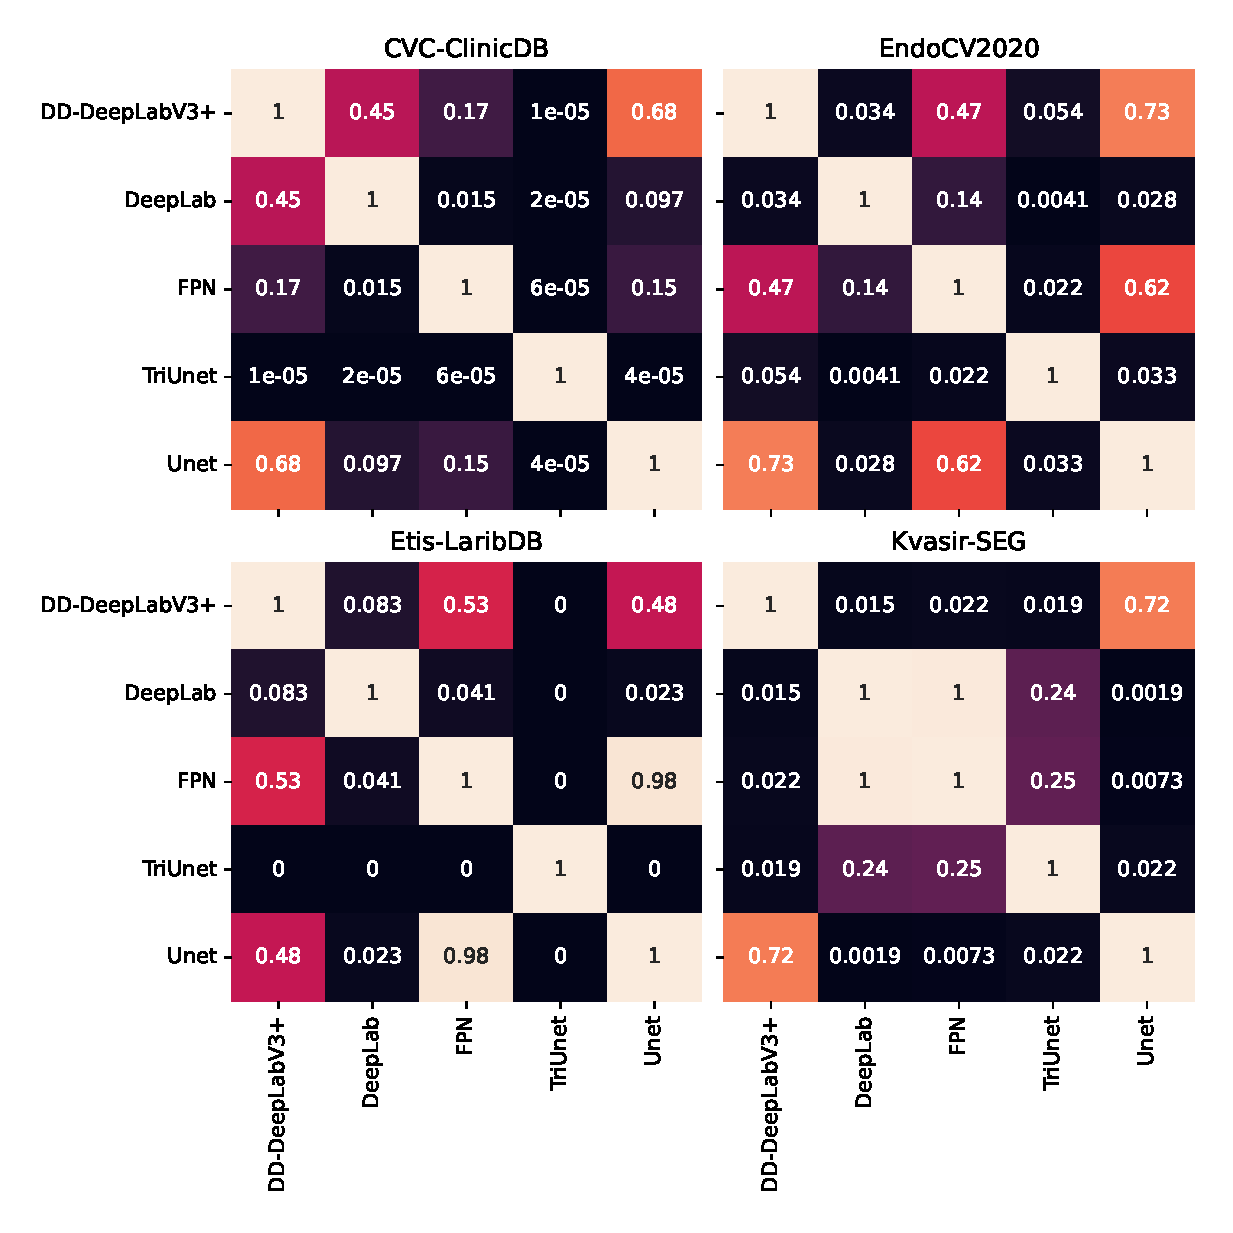
\includegraphics[width=\linewidth]{illustrations/model_pvals.eps}
    \caption{Two-sided independent t-test p-values between models for all datasets}
    \label{models_pvalues}
\end{figure}
% inpainter
\begin{table}[htb]
    \centering
    \begin{tabularx}{\linewidth}{lXXXX}
    \toprule
     Model & CVC-ClinicDB & EndoCV2020 & Etis-LaribDB & Kvasir-SEG\\
    \midrule
    DD-DeepLabV3+ & 0.04454 & 0.95857 & 0.12809 & 0.30201\\ 
    DeepLab & \textbf{0.0096} & 0.08898 & 0.11401 & 0.31065\\ 
    FPN & 0.13769 & 0.95284 & 0.17806 & 0.16613\\ 
    TriUnet & 0.13412 & 0.31111 & 0.19913 & 0.91489\\ 
    Unet & 0.01069 & 0.15406 & 0.02715 & 0.36489\\ 
      \bottomrule
    \end{tabularx}
    \caption[T-test results inpainting]{p-values for each model and dataset between the IoUs of the given models trained with  versus when trained with conventional data augmentation versus models trained with the inpainter as a component of the data augmentation strategy}
    \label{tab:ttest_per_dataset_inpainter}
\end{table}
\begin{table}[htb]
    \centering
    \begin{tabularx}{\linewidth}{lXr}
        \toprule
        Dataset & U-Statistic & p-Value \\
        \midrule
            Kvasir-SEG & 763.0, p=0.15972 \\ 
            Etis-LaribDB & 545.0, p=0.00163 \\ 
            EndoCV2020 & 851.0, p=0.4169 \\ 
            CVC-ClinicDB & 520.0, p=0.00077 \\ 
        \bottomrule
    \end{tabularx}
    \caption[Mann-Whitney U-test results inpainter averaged across models]{Results from Mann-Whitney U-test for each dataset when comparing the average \glspl{iou} of all models trained with conventional data augmentation versus models trained with the inpainter as a component of the data augmentation strategy}
    \label{tab:ttest_avgs_inpainter}
\end{table}

% consistency training
\begin{table}[htb]
    \centering
    \begin{tabularx}{\linewidth}{lXXXX}
    \toprule
      Model & CVC-ClinicDB & EndoCV2020 & Etis-LaribDB & Kvasir-SEG\\
      \midrule
      DD-DeepLabV3+ & 0.014 & 0.985 & 0.083 & 0.170\\
      DeepLab       & 0.029 & 0.901 & \textbf{0.003} & 0.444\\
      FPN           & \textbf{0.004} & 0.038 & \textbf{0.005} & 0.939\\
      TriUnet       & 0.211 & 0.024 & 0.141 & 0.330\\
      Unet          & \textbf{0.000} & \textbf{0.001} & \textbf{0.006} & 0.899\\
      \bottomrule
    \end{tabularx}
    \caption[T-test results consistency training]{p-values for each model and dataset between the IoUs of the given models trained with consistency training versus when trained with data augmentaion}
    \label{tab:ttest_per_dataset_consistency}
\end{table}
\begin{table}[htb]
    \centering
    \begin{tabularx}{\linewidth}{lXr}
            \toprule
            Dataset & U-Statistic & p-Value \\
            \midrule
            Kvasir-SEG & 1066.0 & 0.10293 \\
            Etis-LaribDB & 624.0 & 0.00001\\
            CVC-ClinicDB & 751.0& p=0.00029 \\
            EndoCV2020 & 774.0 & 0.00052    \\
            \bottomrule
        \end{tabularx}
        \caption[Mann-Whitney U-test results consistency training averaged across models]{Results from a Mann-Whitney U-test for each dataset when comparing the average \glspl{iou} across models for Consistency Training vs conventional data augmentation}
        \label{tab:ttest_avgs_consistency}
    \end{table}
    
% Ensembles
\begin{table}[]
    \centering
  \begin{tabularx}{\linewidth}{lXXXX}
    \toprule
    Training method & CVC-ClinicDB & EndoCV2020 & Etis-LaribDB& Kvasir-SEG \\
    \midrule
    No Augmentation             & 0.000 & 0.000 & 0.006 & 0.000 \\ 
    Conventional Augmentation   & 0.000 & 0.000 & 0.003 & 0.000 \\ 
    Consistency Training        & 0.000 & 0.000 & 0.003 & 0.000 \\
    \bottomrule
\end{tabularx}
    \caption{p-values from a Mann-Whitney U-test for each dataset and training method when comparing the mean \gls{iou} of ensembles vs. the mean \gls{iou} across its constituent models.}
    \label{tab:ensemble_v_singular}
\end{table}


\begin{figure}[htb]
    \centering
    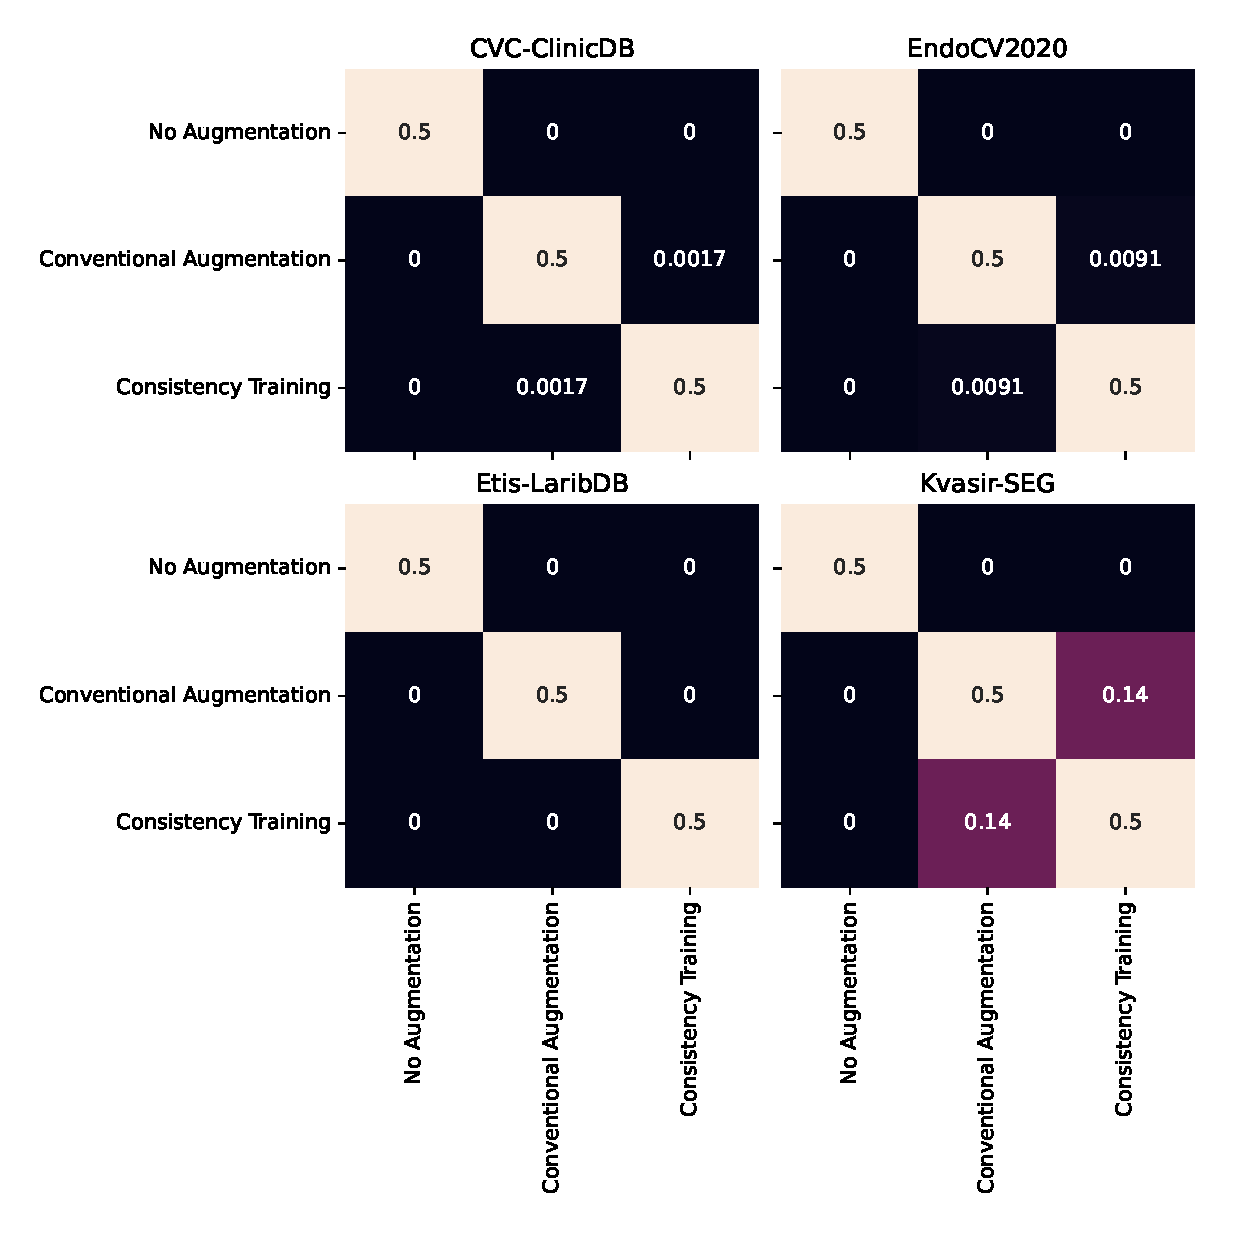
\includegraphics[width=\linewidth]{illustrations/ensemble_relative_pvals.eps}
    \caption[Mann-Whitney U-test results ensembles]{Results from Mann-Whitney U-test for each dataset when comparing the average \glspl{iou} across models for the three training methods. Precision limited to 5 significant figures}
    \label{fig:ttest_training_methods_ensembles}
\end{figure}
    

\newpage
\chapter*{Appendix C: Non-weighted Consistency Training}\label{non_weighted_ctraining}
\addcontentsline{toc}{chapter}{Appendix C: Non-weighted Consistency Training}

\begin{figure}[htb]
    \centering
    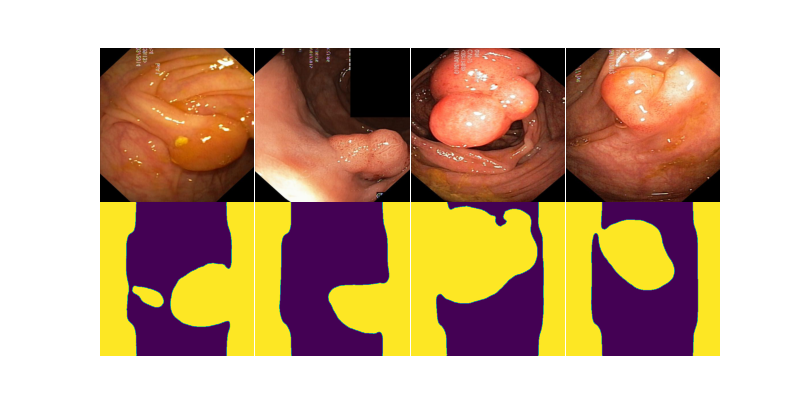
\includegraphics[width=\linewidth]{illustrations/artefacts.png}
    \caption[Unweighted Consistency example]{When the consistency term is not modulated dynamically, the model can quickly learn to predict artifacts around the edges of the image. As polyps can rarely be found in these regions, the consistency term is minimized by predicting consistently wrong predictions where there typically are not polyps. }
    \label{fig:non_weighted_ctraining}
\end{figure}

\chapter*{Appendix D: Paper submitted to NeurIPS2022} \label{Paper}
\addcontentsline{toc}{chapter}{Appendix D: Paper submitted to NeurIPS2022}
\setcounter{chapter}{8}
\setcounter{section}{0}
\setcounter{chapter}{0}
\setcounter{section}{0} 
\includepdf[pages=-]{2022_NIPS_paper_Birk.pdf} 

